\section{Overview}

\subsection{A Story in Pictures}
\begin{frame}
  \centering
  
\includegraphics[height=0.95\textheight]{phd1531}
  \footnote{http://phdcomics.com/comics/archive.php?comicid=1531}
\end{frame}

\begin{frame}
  \centering
  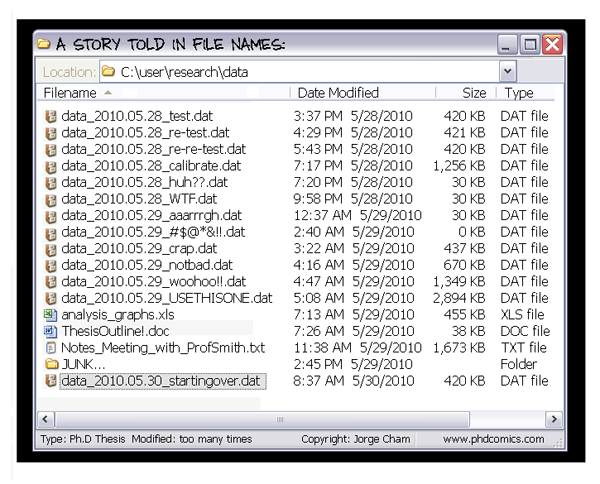
\includegraphics[height=0.95\textheight]{phd1323}
  \footnote{http://phdcomics.com/comics/archive.php?comicid=1323}
\end{frame}

\subsection{Tracking History}

\begin{frame}
  \frametitle{Tracking Changes}
  \begin{itemize}
    \item The history of a project can be viewed as a series of changes:
      \begin{itemize}
        \item A unique identifier
        \item What changed?
        \item When did it change?
        \item Who changed it?
        \item Why did it change?
      \end{itemize}
    \item[]
    \item Difficult to manually track multiple files
  \end{itemize}
\end{frame}

\begin{frame}
  \frametitle{Git: A Version Control System}
  A snapshot of the working directory is taken and \emph{commit}ed to the git data base.
  \begin{itemize}
    \item Unique identifier
      \begin{itemize}
        \item SHA-1 (determined by the files, the author, date, description of change, and the prior history)
      \end{itemize}
    \item What changed \begin{itemize} \item  git diff \end{itemize}
    \item Who changed it \begin{itemize} \item git blame \end{itemize}
    \item Why did it change \begin{itemize} \item git log \end{itemize}
    \item[]
    \item for example:
  \end{itemize}
\end{frame}

\begin{frame}[t,fragile]
  \tiny
  \inputminted{text}{eglog.log}
\end{frame}

\begin{frame}[t,fragile]
  \frametitle{What changed?}
  \small
  \inputminted{text}{egdiff}

  \normalsize
  \begin{itemize}
    \item Diffs are easier to see in several GUI thanks to color coding. More on
      this later.
  \end{itemize}
\end{frame}

\begin{frame}[t,fragile]
  \frametitle{Skipping over errors}
  \small
  \inputminted[firstline=1,lastline=10]{text}{eglog.log}
\end{frame}

\subsection{Overview of Git}

\begin{frame}
  \frametitle{Local Version Control System}
  %\includegraphics[height=0.9\textheight]{}
\end{frame}
